% Title: gl2ps_renderer figure
% Creator: GL2PS 1.4.2, (C) 1999-2020 C. Geuzaine
% For: Octave
% CreationDate: Fri Sep 17 21:56:23 2021
\setlength{\unitlength}{1pt}
\begin{picture}(0,0)
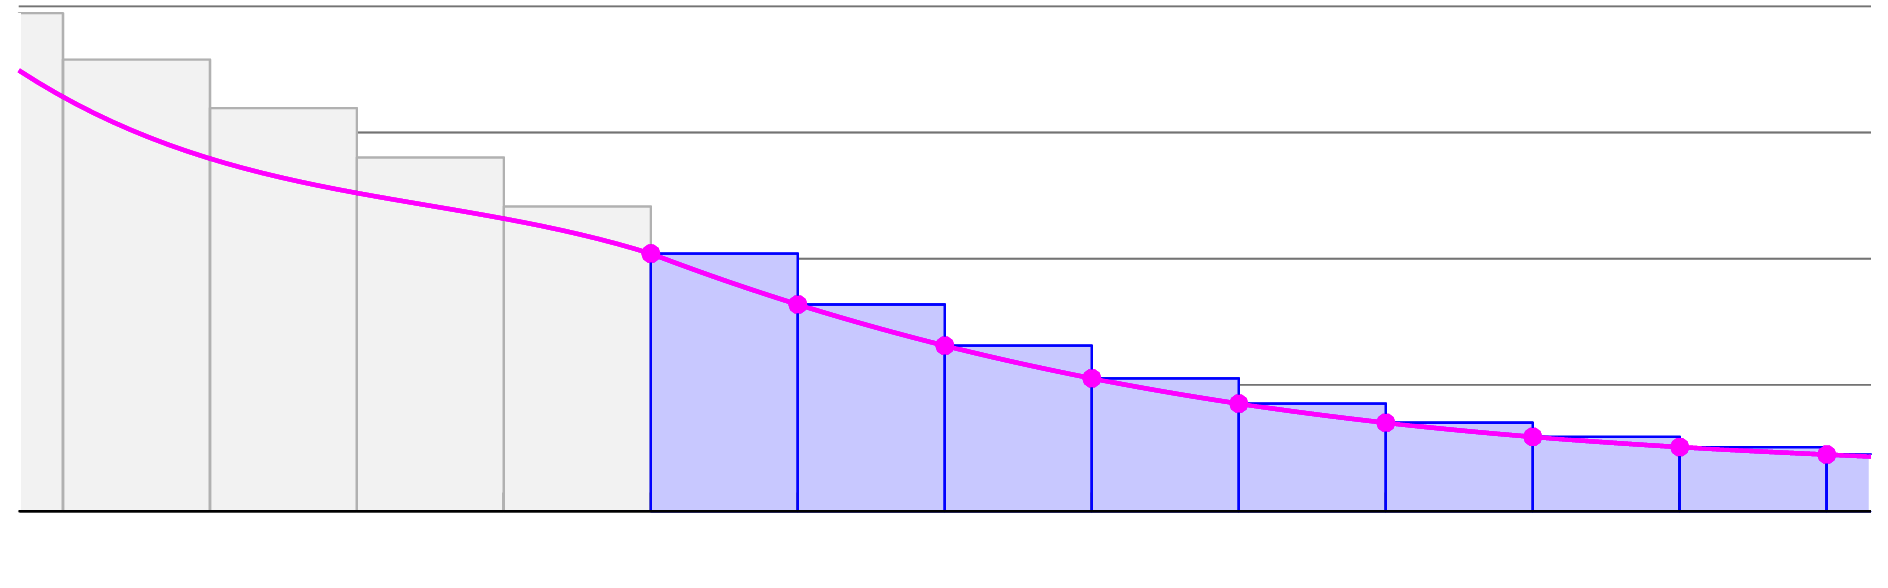
\includegraphics[width=16cm,height=5cm]{fig_teste_integral_right}
\end{picture}%
\begin{picture}(453,141)(0,0)
\fontsize{10}{0}\selectfont\put(120.945,10.9531){\makebox(0,0)[t]{\textcolor[rgb]{0.15,0.15,0.15}{{$N\!-\!1$}}}}
\fontsize{10}{0}\selectfont\put(156.22,10.9531){\makebox(0,0)[t]{\textcolor[rgb]{0.15,0.15,0.15}{{$N$}}}}
\fontsize{10}{0}\selectfont\put(191.496,10.9531){\makebox(0,0)[t]{\textcolor[rgb]{0.15,0.15,0.15}{{$N\!+\!1$}}}}
\fontsize{10}{0}\selectfont\put(262.047,10.9531){\makebox(0,0)[t]{\textcolor[rgb]{0.15,0.15,0.15}{{$N\!+\!3$}}}}
\fontsize{10}{0}\selectfont\put(332.598,10.9531){\makebox(0,0)[t]{\textcolor[rgb]{0.15,0.15,0.15}{{$N\!+\!5$}}}}
\fontsize{10}{0}\selectfont\put(403.15,10.9531){\makebox(0,0)[t]{\textcolor[rgb]{0.15,0.15,0.15}{{$N\!+\!7$}}}}
\end{picture}
